The \verb+VGA_Driver+ module exists to handle the rendering of a 640x480 resolution image and the bar-graphs on the VGA display. The image being rendered consists of a background image previously stored in the SRAM consisting of prefilled bars that within the module will be blanked out according to the input stimuli, which will give the appearance of bars being filled to different levels.   

To render an image on the VGA screen, five main signals is needed. Three analog color channels (red, green and blue) and two signals for synchronization \verb=hsync= and \verb=vsync=. The image is rendered pixel by pixel line by line using a horizontal sweep pattern which is reset by the two sync signals. If a color is set when the sweep resets arbitrary patterns can occur and therefore the signal has to be blanked during the reset phase. This module will be a modified copy of the module used in \emph{Laboration 3}.

%The module \verb+VGA_drive+ has four input signals and five output signals described in table \ref{tab:vgaio}. It consists of eleven sub modules which can be over viewed in \ref{fig:VGAdrive} described below.

\subsection{VGA\_Driver:Bar\_Tender and Bar\_Mixer}\label{sec:Bar_Tender}
\verb+Bar_Tender+ is the submodule responsible for rendering the bar graphs displaying volume, balance and signal strength before and after signal manipulation. The background image already has the bars drawed filled and to give the appearance of them being filled to different levels pixels will be blanked out from the top down. Using \verb=volume, balance, bar, new_bar= and \verb=pixelindex=, \verb+Bar_Tender+ will calculate which pixels should be blanked and set the signal \verb=render_bar= high.

\verb+Bar_Mixer+ works as a multiplexer blanking out the bars. The color information is passed through if \verb=render_bar= signal is low and blanks out the pixel if high, which gives the effect of bar graphs being filled.

\begin{figure}[H]
  \centering
  \caption{List of input and output signals (\texttt{VGA\_Driver})}
  \label{tab:vgaio}
    \begin{tabular}{|l|c|l|}
      \hline
      Name & Type & Description \\
      \hline
      \verb+volume_input+ & Input & A 4-bit input containing volume information\\
      \hline
      \verb+balance_input+ & Input & A 4-bit input containing balance information\\
      \hline
      \verb+{L,R}bar+ & Input & A 8-bit input containing signal sound input signal level\\
      \hline
      \verb+{L,R}new_bar+ & Input & A 8-bit input containing manipulated input signal level\\
      \hline
   	\verb+vsync+ & Output & Control signal for reading the analysis registers\\
      \hline
      %  \verb=render_bars= & Out/In & Control signal for \verb=Bar_Mixer=\\
      % \hline
      %\verb+VGA_blank+ & Output & A blanking signal for blanking when resetting scan\\
      %\hline
      %\verb+vga_{r,g,b}+ & Output & Three signals containing color information\\
      \hline
    \end{tabular}
\end{figure}
\begin{figure}[H]
        \centering
        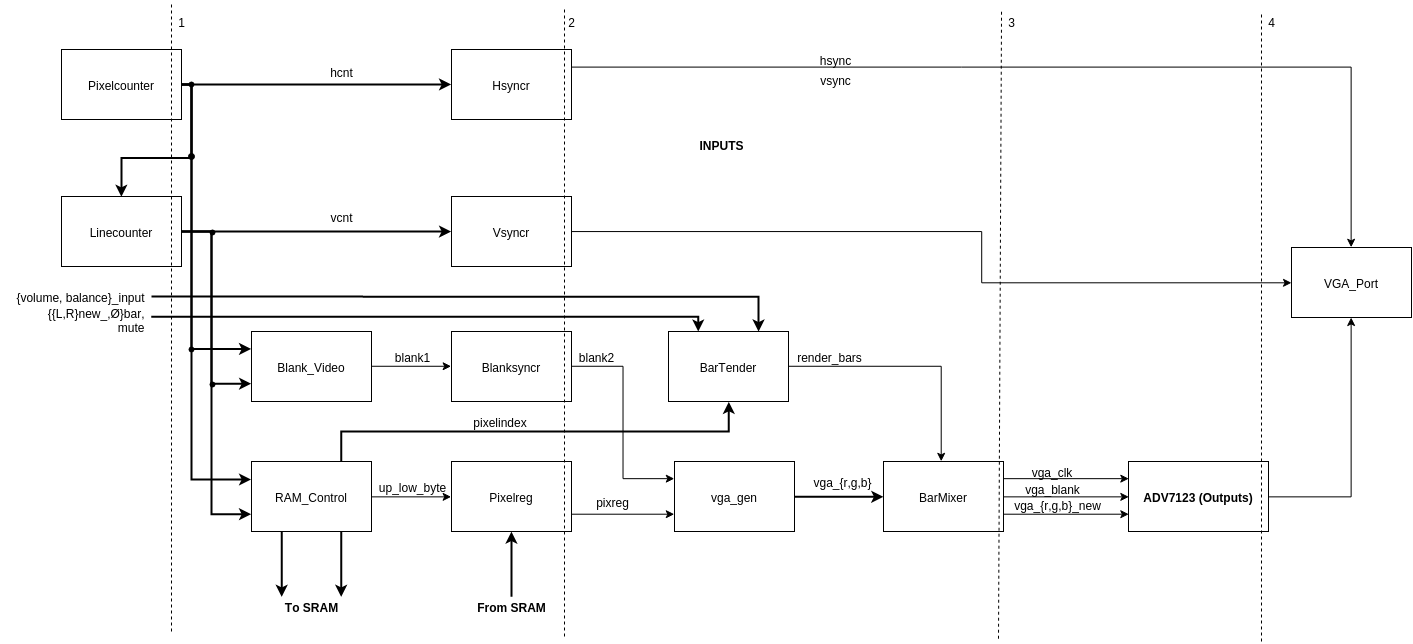
\includegraphics[width=15cm]{vgadrive.png} 
        \caption{Block diagram of \texttt{VGA\_Driver}}
        \label{fig:VGAdrive}
\end{figure}

%\subsection{VGA\_Driver:Pipelining}
%Since there is a time delay for the system to calculate ram address, generate \verb=pixel_index= the system is pipelined. The four pipe-line stages are illustrated with dashed lines in figure \ref{fig:VGAdrive}. This means that there is a time delay of 3 clock cycles between which pixel is handled and which is drawn. 

%\subsection{VGA\_Driver:Pixelcounter} 
%The sub module \verb+Pixelcounter+ is a generating the internal 10 bit signal \verb=hcount=. \verb=hcount= functions as a \verb+Pixelcounter+ for each row and will count from 0 to 797 which represent the pixels needed for each row in the scanning. 
 
%\subsection{VGA\_Driver:Linecounter}
%\verb+Linecounter+ works almost the same as \verb=Pixelcounter= and generates the signal \verb=vcount=. \verb=vcount= is incremented with one every time \verb=hcount= resets and resets after reaching 525. This makes \verb=hcount= and \verb=vcount= together act as coordinates to each pixel on the screen during the scanning.

%\subsection{VGA\_Driver:Clock\_Divider}
%\verb+Clock_Divider+ is just as its name suggests a clock divider which divides the system clock of 50 MHz to 25 MHz. This is needed because the timings in the VGA-interface for the resolution used requires a clock of 25 MHz. 

%\subsection{VGA\_Driver:Blank\_Video}

%Due to the nature of the sweep in the VGA-interface the signal needs to be blanked just before, during and after the synchronization signals. This is done using the \verb=Blank_Video= sub module, the 1 bit blanking signal is active low and should therefore be zero while outside of the visible image and and one inside. This is done by setting \verb=blank= high when \verb=hsync= is between 0 and 639 and \verb=vsync= is between 0 and 479.    


%\subsection{VGA\_Driver:RAM\_Control}
%The image used as a background is pre-stored in the SRAM and to acess the image data we need to generate some signals to the SRAM. The control signals \verb=CE, OE, WE, UB, LB= are set constant to 0, 0, 1, 0, 0, which means that SRAM should be enabled read-only and access both upper and lower byte.

%Each 16 bit row in the SRAM contains color information about two pixels, one in the lower and one in the upper byte. Therefore we must generate two signals: \verb=sram_addr= which provides the SRAM with the correct adress and \verb=up_lo_byte= that provides the sub module Pixelreg with the information about which of the bytes should be read. It also generates the output \verb=pixelindex= which is a counter that counts each pixel in the visible area used by \verb=Bar_Tender= (see section \ref{Bar_Tender}).   

%This module is identic to the \verb=RAM_Control= module in the third laboration with the exception of \verb=pixelindex=, which is a counter for each pixel in the visible area. It is used by \verb=Bar_Tender= (see section \ref{sec:Bar_Tender}

%\subsection{VGA\_Driver:Hsyncr, Vsyncr}
%The sub modules \verb+Hsyncr+ and \verb+Vsyncr+ are responsible for generating the \verb=hsync= and \verb=vsync= signals used for resetting the sweep. In the resolution used in this application this means that \verb=hsync= should be active(low) during hcount values between 490 and 493 and \verb=vsync= between \verb=vcount= values of 655 and 750.   

%\subsection{blank\_syncr}
%\verb=blank_syncr= is a single d-flip flop needed for pipelining.

%\subsection{VGA\_Driver:pixel\_reg}
%\verb=Pixelregister= is responsible for reading the image information from SRAM, the image information is avaliable on the SRAM-bus and the module simply needs to read the correct byte (using \verb=up_lo_byte=) and put it in a pipeline register.

%\subsection{VGA\_Driver:VGA\_gen}
%\verb+VGA_gen+ will take the \verb=pix_reg= register and supply it to the three color channel outputs \verb=VGA_r=, \verb=VGA_g= and \verb=VGA_b=. Due to the fact that the AVD7123 chip expects 10 bit values and the stored image containing 3-bit color values the values need to be scaled up before provided to \verb+Bar_Mixer+.


